

\documentclass[class=article, crop=true]{standalone}
\usepackage{subcaption}
\usepackage[subpreambles=true]{standalone}
\usepackage{tikz}
\usepackage{amssymb}
\usepackage{amsmath}
\usetikzlibrary{arrows.meta, positioning}

\begin{document}

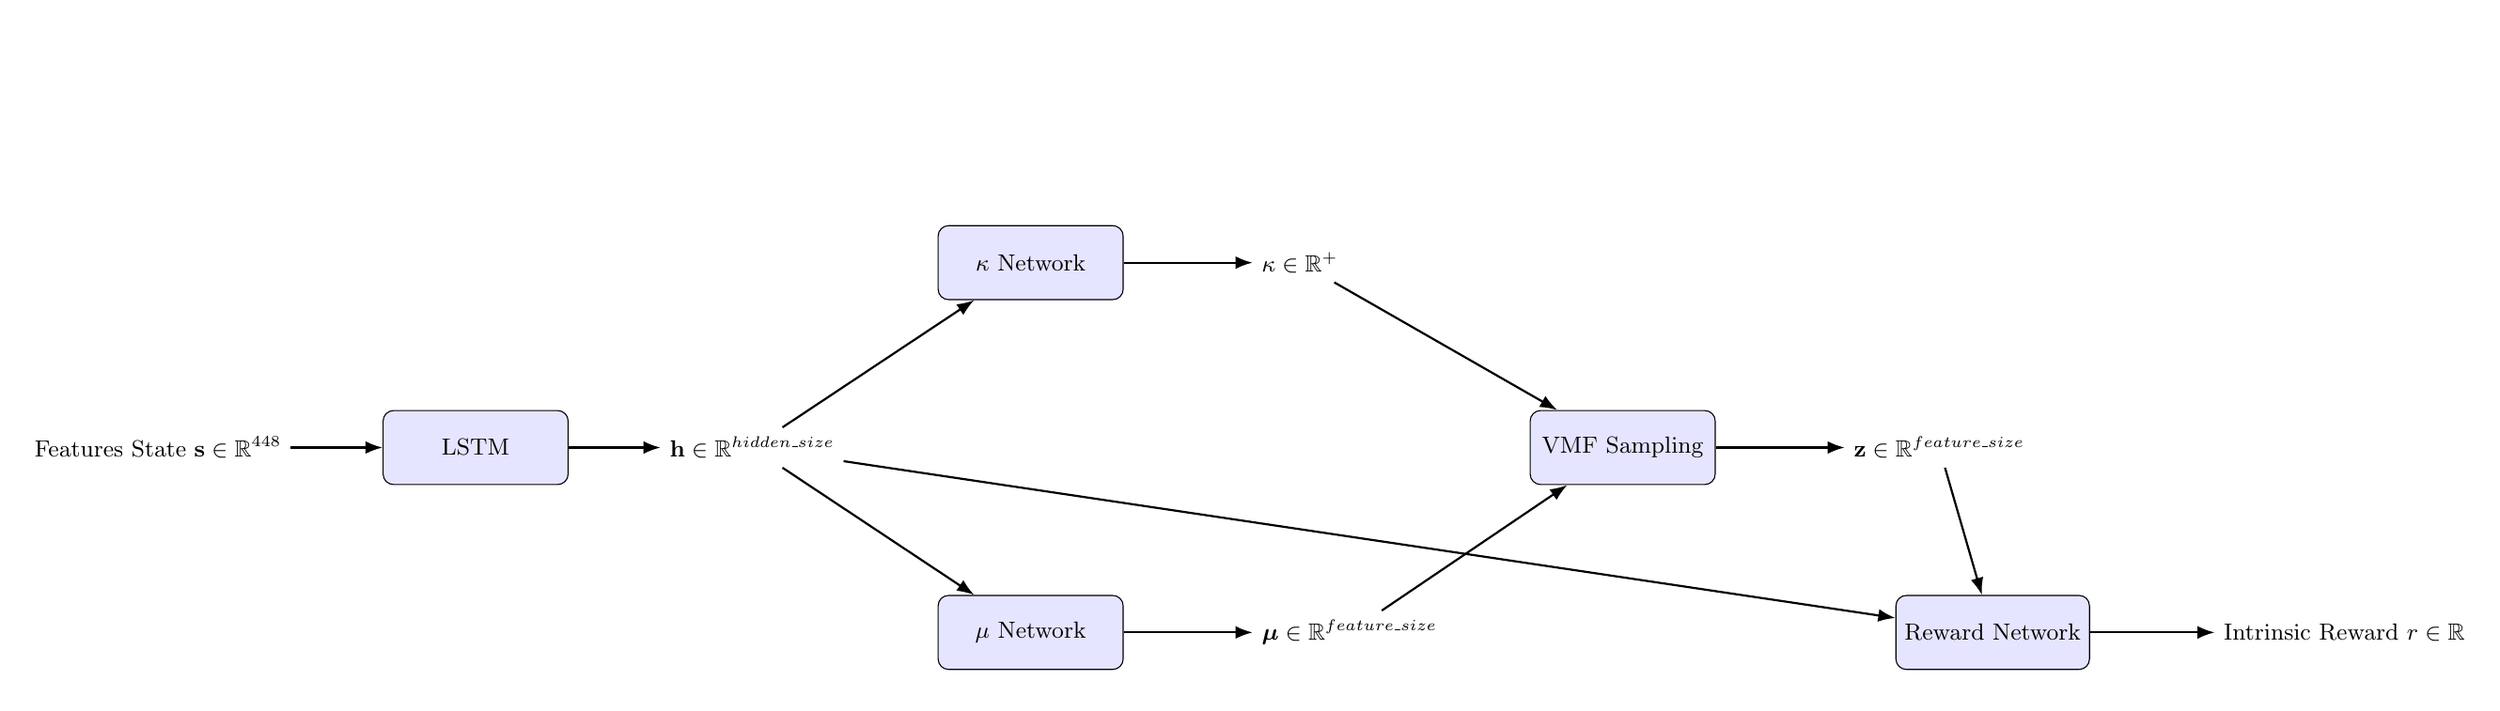
\begin{tikzpicture}[
    op/.style={rectangle, draw, rounded corners, text centered, minimum height=1cm, minimum width=2.5cm, font=\small, fill=blue!10},
    tensor/.style={font=\small},
    arrow/.style={-{Latex}, thick}
]

% Background
\fill[white] (-13.2, -3.2) rectangle (18.1, 5.7);

% Input state
\node[tensor, anchor=east] (state) at (-10, 0) {Features State $\textbf{s} \in \mathbb{R}^{448}$};

% LSTM
\node[op] (lstm) at (-7.5, 0) {LSTM};
\node[tensor, anchor=west] (hidden) at (-5, 0) {$\textbf{h} \in \mathbb{R}^{hidden\_size}$};

% Mu network branch
\node[op] (mu_net) at (0, -2.5) {$\mu$ Network};
\node[tensor, anchor=west] (mu) at (3, -2.5) {$\boldsymbol{\mu} \in \mathbb{R}^{feature\_size}$};

% Kappa network branch
\node[op] (kappa_net) at (0, 2.5) {$\kappa$ Network};
\node[tensor, anchor=west] (kappa) at (3, 2.5) {$\kappa \in \mathbb{R}^+$};

% VMF sampling
\node[op] (vmf) at (8, 0) {VMF Sampling};
\node[tensor, anchor=west] (z) at (11, 0) {$\textbf{z} \in \mathbb{R}^{feature\_size}$};

% Reward network
\node[op] (reward_net) at (13, -2.5) {Reward Network};
\node[tensor, anchor=west] (reward) at (16, -2.5) {Intrinsic Reward $r \in \mathbb{R}$};

% Connections
\draw[arrow] (state) -- (lstm);
\draw[arrow] (lstm) -- (hidden);
\draw[arrow] (hidden) -- (mu_net);
\draw[arrow] (hidden) -- (kappa_net);
\draw[arrow] (mu_net) -- (mu);
\draw[arrow] (kappa_net) -- (kappa);
\draw[arrow] (mu) -- (vmf);
\draw[arrow] (kappa) -- (vmf);
\draw[arrow] (vmf) -- (z);
\draw[arrow] (z) -- (reward_net);
\draw[arrow] (hidden) -- (reward_net);
\draw[arrow] (reward_net) -- (reward);

\end{tikzpicture}


 





% \begin{tikzpicture}[node distance=1.5cm and 2cm]

% % Time steps
% \node[mynode, fill=blue!20] (lstm_t1) {LSTM $t_1$};
% \node[mynode, fill=blue!20, right=3cm of lstm_t1] (lstm_t2) {LSTM $t_2$};
% \node[mynode, fill=blue!20, right=3cm of lstm_t2] (lstm_t3) {LSTM $t_3$};

% % Rewards and outputs
% \node[mynode, fill=red!20, above=1.5cm of lstm_t1] (reward_t1) {Reward $r_{t+1}$};
% \node[mynode, fill=red!20, above=1.5cm of lstm_t2] (reward_t2) {Reward $r_{t+2}$};
% \node[mynode, fill=red!20, above=1.5cm of lstm_t3] (reward_t3) {Reward $r_{t+3}$};

% % mu and z
% \node[mynode, fill=green!20, below=1.5cm of lstm_t1] (mu_t1) {$\mu_{t}$};
% \node[mynode, fill=yellow!20, below right=1.5cm and 1cm of mu_t1] (z_t1) {$z_{t}$};

% \node[mynode, fill=green!20, below=1.5cm of lstm_t2] (mu_t2) {$\mu_{t+1}$};
% \node[mynode, fill=yellow!20, below right=1.5cm and 1cm of mu_t2] (z_t2) {$z_{t+1}$};

% \node[mynode, fill=green!20, below=1.5cm of lstm_t3] (mu_t3) {$\mu_{t+2}$};
% \node[mynode, fill=yellow!20, below right=1.5cm and 1cm of mu_t3] (z_t3) {$z_{t+2}$};

% % Connections between time steps
% \draw[arrow] (lstm_t1) -- (reward_t1);
% \draw[arrow] (lstm_t2) -- (reward_t2);
% \draw[arrow] (lstm_t3) -- (reward_t3);

% \draw[arrow] (lstm_t1) -- (mu_t1);
% \draw[arrow] (mu_t1) -- (z_t1);
% \draw[arrow] (z_t1) -- (reward_t1);

% \draw[arrow] (lstm_t2) -- (mu_t2);
% \draw[arrow] (mu_t2) -- (z_t2);
% \draw[arrow] (z_t2) -- (reward_t2);

% \draw[arrow] (lstm_t3) -- (mu_t3);
% \draw[arrow] (mu_t3) -- (z_t3);
% \draw[arrow] (z_t3) -- (reward_t3);

% % Backprop connections
% \draw[arrow, dashed, red] (reward_t3.north) -- +(0,1);
% \draw[arrow, dashed, red] (reward_t2.north) -- +(0,1);
% \draw[arrow, dashed, red] (reward_t1.north) -- +(0,1);

% \end{tikzpicture}


\end{document}